\documentclass[
  captions=tableheading,
  bibliography=totoc, 
  titepage=firstiscover,
]{scrartcl}

\usepackage{blindtext} %neuer input

\usepackage{longtable} % Tabellen über mehrere Seiten

\usepackage[utf8]{inputenc} %neuer input

\usepackage{scrhack}

\usepackage[aux]{rerunfilecheck} %Warnung falls nochmal kompiliert werden muss

\usepackage{fontspec} %Fonteinstellungen

\recalctypearea{}

\usepackage[main=ngerman]{babel} %deutsche Spracheinstellung

\usepackage{ragged2e} %neuer input

\usepackage{amsmath, nccmath}

\usepackage{amssymb} %viele mathe Symbole

\usepackage{mathtools} %Erweiterungen für amsmath


\DeclarePairedDelimiter{\abs}{\lvert}{\rvert}
\DeclarePairedDelimiter{\norm}{\lVert}{\rVert}

\DeclarePairedDelimiter{\bra}{\langle}{\rvert}
\DeclarePairedDelimiter{\ket}{\lvert}{\rangle}

\DeclarePairedDelimiterX{\braket}[2]{\langle}{\rangle}{
#1 \delimsize| #2
}

\NewDocumentCommand \dif {m}
{
\mathinner{\symup{d} #1}
}


\usepackage[
  math-style=ISO,
  bold-style=ISO,
  sans-style=italic,
  nabla=upright,
  partial=upright,
  warnings-off={
    mathtools-colon,
    mathtools-overbracket,
  },
]{unicode-math}

\setmathfont{Latin Modern Math}
\setmathfont{XITS Math}[range={scr, bfscr}]
\setmathfont{XITS Math}[range={cal, bfcal}, StylisticSet=1]


\usepackage[
  locale=DE,
  separate-uncertainty=true,
  per-mode=reciprocal,
  output-decimal-marker={,},
]{siunitx}

\usepackage[autostyle]{csquotes} %richtige Anführungszeichen

\usepackage{xfrac}

\usepackage{float}

\floatplacement{figure}{htbp}

\floatplacement{table}{htbp}

\usepackage[ %floats innerhalb einer section halten
  section,   %floats innerhalb er section halten
  below,     %unterhalb der Section aber auf der selben Seite ist ok
]{placeins}

\usepackage[
  labelfont=bf,
  font=small,
  width=0.9\textwidth,
]{caption}

\usepackage{subcaption} %subfigure, subtable, subref

\usepackage{graphicx}

\usepackage{grffile}

\usepackage{booktabs}

\usepackage{microtype} %Verbesserungen am Schriftbild

\usepackage[
backend=biber,
]{biblatex}

\addbibresource{../lit.bib}

\usepackage[ %Hyperlinks im Dokument
  german,
  unicode,
  pdfusetitle,
  pdfcreator={},
  pdfproducer={},
]{hyperref}

\usepackage{bookmark}

\usepackage[shortcuts]{extdash}

%\usepackage{warpcol}


\begin{document}
    \title{V354 Gedämpfte und erzwungene Schwingungen}
    \author{  
    Tobias Rücker\\
    \texorpdfstring{\href{mailto:tobias.ruecker@tu-dortmund.de}{tobias.ruecker@tu-dortmund.de}
    \and}{,} 
    Paul Störbrock\\
    \texorpdfstring{\href{mailto:paul.stoerbrock@tu-dortmund.de}{paul.stoerbrock@tu-dortmund.de}}{}
    }
    \date{Durchführung: 26.11.2019, Abgabe: 03.12.2019\vspace{-4ex}}
\maketitle
\center{\Large Versuchsgruppe: \textbf{42}}
    
    \begin{abstract}
    \centering
        \textbf{Ziel:} 
    \end{abstract}

\newpage
\tableofcontents
\newpage

% Theorie %%%%%%%%%%%%%%%%%%%%%%%%%%%%%%%%%%%%%%%%%%%%%%%%%%%%%%%%%%%%%%%%%%%%%%%%%%%%%%%%%%%%%%%%%%%%%%%%%%%%%%%%%%%%%%%%%%%%%%%%%%%%%%%%%%%%%%%%%%%

\section{Theorie}\justifying
\begin{align}
\intertext{Ein Schwingkreis beschreibt einen Schaltkreis bestehend aus einem
Kondensator und einer Spule. Die Spule besitzt dabei die Induktivität $L$ und der
Kondensator die Kapazität $C$. Wird auf diese Schaltung nun eine Spannung $U_0$ 
gegeben, so oszilliert der Schwingkreis und führt eine ungedämpfte Schwingung aus. 
Wird nun ein Widerstand in die Schaltung eingebaut, so verliert das System mit der
Zeit Energie, die in Form von Joulscher Wärme an den Widerstand irreversibel
übertragen wird. Dadurch führt das System eine gedämpfte Schwingung aus.
Die zeitliche Veränderung der Stromstärke kann dabei durch folgende Formel
beschrieben werden \cite{V354}:}
\symbffrak{I}(t) &= \symbffrak{U}_1e^ {i\tilde{\omega}_1 t}+\symbffrak{U}_2 e^{i \tilde{\omega}_2 t} \text{, wobei}\\
\tilde{\omega} _{1,2} &= i\frac{R}{2L} \pm \sqrt{\frac{1}{LC}-\frac{R^2}{4L^2}} \label{eq:omega}\\
\intertext{Aus diesem Zusammenhang ergeben sich drei verschiedene Fälle.
Der erste Fall beschreibt, dass \cite{V354}}
\frac{1}{LC} & > \frac{R^2}{4L^2} \label{eq:Fall1}
\intertext{ist und damit der Wurzelterm von $\tilde{\omega}$ \eqref{eq:omega} komplex wird.
Die zugehörige Schwingungsgleichung entspricht damit \cite{V354}}
    I(t)&=A_0 e^{-2 \pi \mu t} \cos (2 \pi \nu t + \eta) \label{eq:I}
\end{align}
\justifying
Diese Gleichung beschreibt eine ungedämpfte Schwingung. Die Amlitude $A_0$ läuft dabei
exponentiell gegen null.
Die Schwingungsdauer lässt sich dabei für diesen Fall schreiben als \cite{V354}:
\begin{align}
    T_0 &\phantom{:}=\frac{2 \pi}{\omega _0}=2 \pi \sqrt{LC} \text{, wobei sich nach einer Zeit $T_{ex}$} mit\\
    T_{ex}&:= \frac{1}{2 \pi \mu}=\frac{2L}{R} \label{eq:Abkling}
\end{align}
\justify
die Spannungsamplitude um den Faktor $\sfrac{1}{e}$ verringert hat.
$T_{ex}$ wird daher auch Ablinkdauer genannt.
\justify
Der zweite Fall \cite{V354}
\begin{align}
    \frac{1}{LC} <\frac{R^2}{4L^2} \label{eq:Fall2}
\end{align}
stellt den Kriechfall dar. Bei diesem verschwindet der oszillatorische Teil und
die Wurzel aus Gleichung \eqref{eq:omega} wird positiv.
Die Funktion geht mit maximal einem Nulldurchgang nicht-oszillatorisch gegen null.
Ob ein Nulldurchgang sattfindet hängt dabei von den Anfangsbedingungen ab.
\justify
Der dritte Fall stellt einen Spezialfall des zweiten dar.
Bei diesem ist die Bedingung \cite{V354}:
\begin{align}
    \frac{1}{LC} = \frac{R^2}{4L^2} \label{eq:Fall3}
\end{align}
Dieser wird der aperiodische Grenzfall genannt. Bei diesem kehrt die Kurve
am schnellsten zur Null zurück.\\
Neben gedämpften Schwingungen treten auch häufig erzwungene Schwingungen auf,
die hier durch eine sinusförmige Wechselpannung realisiert wird. 
Die Frequenzabhängigkeit des Kondensators wird dabei durch 
\begin{align}
    U_C (\omega)=\frac{U_0}{\sqrt{(1-LC\omega ^2)^2+\omega ^2 R^2 C^2}}
\end{align}
beschrieben.
Dabei ist zu bemerken, dass diese Funktion ein Maximum besitzt, welches die
angelegte Spannungsamplitude $U_0$ übersteigen kann.\\
Diese Frequenz wird im Allgemeinen als Resonanzfrequenz $\omega_{res}$ \cite{V354} 
\begin{align}
    \omega_{res} = \sqrt{\frac{1}{LC}-\frac{R^2}{2L^2}} \label{eq:omegares}
\end{align}
bezeichnet.\\
Aus dieser Formel können zwei Fälle betrachtet werden.
Für den ersten Fall wird die schwache Dämpfung betrachtet \cite{V354}:
\begin{align}
    \frac{1}{LC} \gg \frac{R^2}{4L^2} \label{eq:Fall1b}
\end{align}
Der Faktor $\sfrac{1}{\omega _0 RC}$ beschreibt in diesem Fall, um welchen Faktor 
$U_{C,\text{max}}$ die Spannung $U_0$ übersteigt. Daher wird er auch als Güte 
oder Resonanzüberhöhung q bezeichnet.
Eine andere Beschreibung von q lässt sich mit der Breite der 
Resonanzkurve finden \cite{V354}:
\begin{align}
    q = \frac{\omega _0}{\omega _+ - \omega _-} \label{eq:guete}
\end{align}
Dabei beschreiben $\omega _+$ und $\omega _-$ die Breite der Resonanzkurve.
Sie beschreiben die Fequenzen, bei denen die Spannung auf die Größe 
$\sfrac{U_{C,\text{max}}}{\sqrt{2}}$ vom Maximum gesunken ist.
Die Breite der Resonanzkurve kann dabei durch
\begin{align}
    \omega _+ - \omega _- \approx \frac{R}{L} \label{eq:om+-}
\end{align}
approximiert werden.\\
Für den Fall der starken Dämpfung \cite{V354}
\begin{align}
    \frac{1}{LC} \ll \frac{R^2}{4L^2} \label{eq:Fall2b}
\end{align}
existiert keine Resonanzüberhöhung mehr. 
Die frenquenzabhängige Phasenverschiebung \cite{V353}
\begin{align}
    \varphi(\nu) &= \frac{\Delta T}{T} \cdot 2 \pi \quad &\text{mit} \; T &= \frac{1}{\nu} \label{eq:nu}
\end{align}
zeigt, dass sich dabei der Wert $\sfrac{\pi}{2}$ bei \cite{V354}
\begin{align}
    \omega _0^2 &= \frac{1}{LC} \label{eq:omega0}
\intertext{ergibt. Wird $\omega _0 $ um $\pm\sfrac{\pi}{4}$ verschoben, so ergeben sich die Werte \cite{V354}}
    \omega_{1,2} &= \pm \frac{R}{2L} + \sqrt{\frac{R^2}{4L^2} + \frac{1}{LC} } \label{eq:om12}
\intertext{für $\omega _1$ und $\omega _2$. Daraus lässt sich die Beziehung \cite{V354}}
    \omega _1 - \omega _2 &= \frac{R}{L} \label{eq:omdiff}
\end{align}
herleiten.

% Fehlerrechnung %%%%%%%%%%%%%%%%%%%%%%%%%%%%%%%%%%%%%%%%%%%%%%%%%%%%%%%%%%%%%%%%%%%%%%%%%%%%%%%%%%%%%%%%%%%%%%%%%%%%%%%%%%%%%%%%%%%%%%%%%%%%%%%%%%%%%%%%%%%

\section{Fehlerrechnung}

Für die Auswertung werden die folgenden Formeln zur Bestimmung der eventuell anfallenden Fehler benötigt:
\begin{subequations}    
\begin{align}
    \intertext{Der Mittelwert}
        \overline{x} &= \frac{1}{N}\sum_{i=1}^{N} x_i \label{eq:mittelw}
    \intertext{Der Fehler des Mittelwerts}
        \Delta\overline{x} &= \frac{1}{\sqrt{N}} \sqrt{\frac{1}{1-N} \sum_{i=1}^{N} (x_i - \overline{x})^2} \label{eq:fmittelw}
    \intertext{Die gaußsche Fehlerfortpflanzung}
        \Delta f &= \sqrt{\sum_{i=1}^{N} \left( \frac{\delta f}{\delta x_i} \right)^2 \cdot (\Delta x_i)^2} \label{eq:ffort}
    \intertext{In der Auswertung selbst wird die Fehlerrechnung mithilfe von Pyhtonbefehlen \cite{uncertainties} durchgeführt.
    Für die lineare und nichtlineare Ausgleichsrechnung werden folgende Funktionen benötigt:}
        y &= m \cdot x + b\\
        m &= \frac{\overline{xy} - \overline{x} \cdot \overline{y}}{\overline{x^2} - {\overline{x}}^2} \qquad \qquad
        b = \frac{\overline{y} \cdot \overline{x^2} - \overline{xy} \cdot \overline{x}}{\overline{x^2} - {\overline{x}}^2}
\end{align}
\end{subequations}

% Aufgaben %%%%%%%%%%%%%%%%%%%%%%%%%%%%%%%%%%%%%%%%%%%%%%%%%%%%%%%%%%%%%%%%%%%%%%%%%%%%%%%%%%%%%%%%%%%%%%%%%%%%%%%%%%%%%%%%%%%%%%%%%%%%%%%%%%%%%%%%%%%

\section{Aufgaben}\justifying

 \begin{enumerate}

    \item[a)] \justifying Zuerst wird mittels der Tabelle \ref{tab:data_a} eine lineare
                          Ausgleichsrechnung durchgeführt und aus dem Ergebnis der effektive
                          Dämpfungswiderstand bestimmt.

    \item[b)] \justifying Anschließend wird über einen variablen Widerstand bestimmt,
                          wo sich der aperiodische Grenzfall befindet. 
  
    \item[c)] \justifying Daraufhin wird die Frequenzabhängigkeit
                          der Kondensatorspanung über einen Plot der Messwertpaare
                          betrachtet.
  
    \item[d)] \justifying Schließlich wird der Zusammenhang zwischen Phase und Frequenz
                          durch eine Messung an einem Serienresonanzkreis bestimmt.
    
  \end{enumerate}

% Versuchsaufbau %%%%%%%%%%%%%%%%%%%%%%%%%%%%%%%%%%%%%%%%%%%%%%%%%%%%%%%%%%%%%%%%%%%%%%%%%%%%%%%%%%%%%%%%%%%%%%%%%%%%%%%%%%%%%%%%%%%%%%%%%%%%%%%%%%%%%%%%%%%

\section{Versuchsaufbau}\justifying
Benötigt werden: \textit{Ein Generator mit einem Innenwiderstand von 2.5$\Omega$, 
ein analoges Zweikanal-Oszilloskop, ein LRC-Glied mit drei ohmschen Widerständen 
($R_1 < R_2$), wovon einer der Widerstände ($R_3$) variabel sein soll, 
zwei BNC-Kabel, eine BNC-Steckverbindung und einen Tastkopf}.\\
Zuerst wird die BNC-Steckverbindung an dem Generator angebracht. 
Dann wird die Steckverbindung mit einem der Widerstände des LRC-Glieds und mit dem zweiten 
Eingang des Oszilloskops verbunden.
Zuletzt wird das LRC-Glied über einem BNC-Kabel mit Tastkopf 
mit dem ersten Eingang des Oszilloskops verbunden.


% Versuchsdurchführung %%%%%%%%%%%%%%%%%%%%%%%%%%%%%%%%%%%%%%%%%%%%%%%%%%%%%%%%%%%%%%%%%%%%%%%%%%%%%%%%%%%%%%%%%%%%%%%%%%%%%%%%%%%%%%%%%%%%%%%%%%%%%%%%%%%%%%%%%%%

\section{Versuchsdurchführung}\justifying

 \begin{enumerate}

    \item[a)] \justifying Zu Beginn wird am Generator eine Frequenz von 100Hz 
    eingestellt und eine Erregerspannung von 10V eingestellt. Danach wird der 
    Generator mit dem kleineren der festen Widerstände verbunden.
    Um die lineare Ausgleichsrechnung der Einhüllenden zu bestimmen, wird
    ein Bild vom Oszilloskop angefertigt aus dem dann Messwerte entnommen werden
    können.

    \item[b)] \justifying Um den Widerstand $R_{ap}$ zu bestimmen, wird der Generator 
    an den maximal eingestellten variablen Widerstand angeschlossen. Anschließend wird 
    der variable Widerstand reduziert, bis am Oszilloskop eine Überschwingung erkennbar 
    wird. Daraufhin wird der Widerstand stetig erhöht bis die Überschwingung verschwindet 
    und der bestimmte Widerstand notiert.
  
    \item[c/d)] \justifying Dann wird für die Messung der Frequenzabhängigkeit
                          der größere Widerstand von 271.6$\pm0.2\Omega$ angeschlossen.
                          Daraufhin werden die Werte für Phase und Frequenz um die 
                          Resonanzfrequenz gemessen und datiert.
  
    

  \end{enumerate}

% Auswertung %%%%%%%%%%%%%%%%%%%%%%%%%%%%%%%%%%%%%%%%%%%%%%%%%%%%%%%%%%%%%%%%%%%%%%%%%%%%%%%%%%%%%%%%%%%%%%%%%%%%%%%%%%%%%%%%%%%%%%%%%%%%%%%%%%%%%%%%%%%

\section{Auswertung}\justifying

%Auswertung 5a ----------------------------------------------------------------------------------------------------------------------------------------

  \begin{figure}[H]
    \begin{subfigure}{0.495\linewidth}
     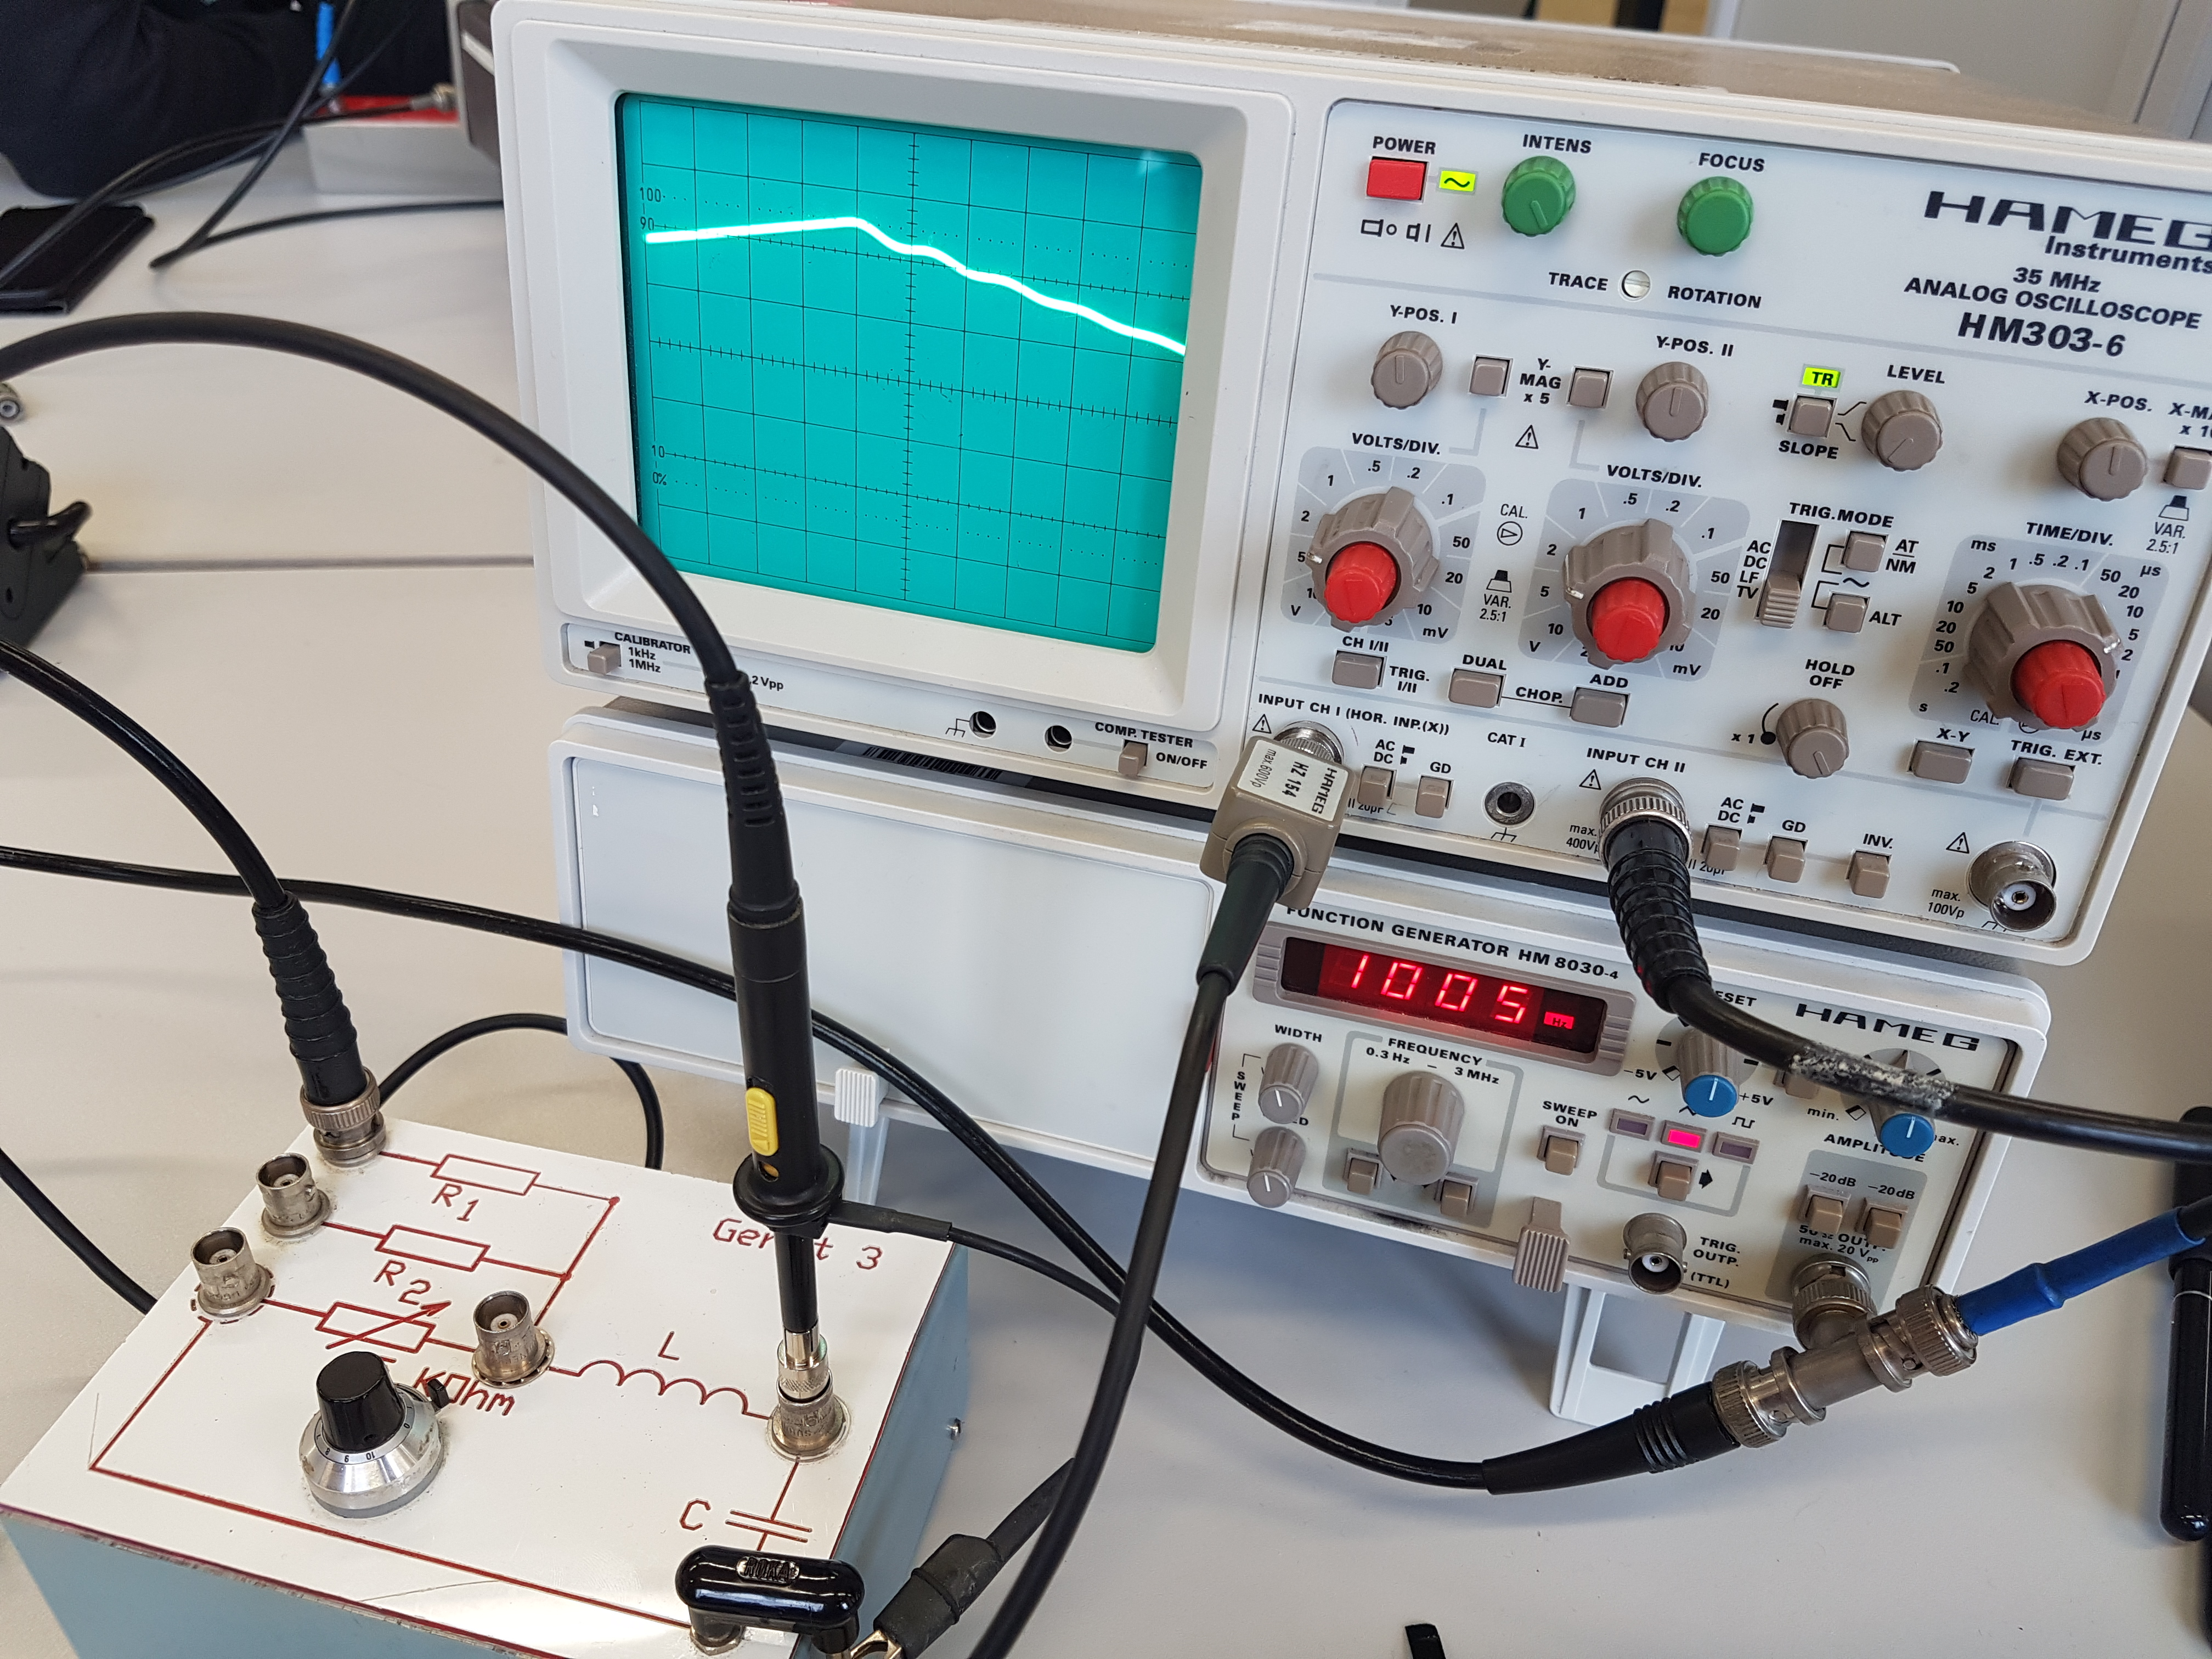
\includegraphics[width=\textwidth]{images/R1.jpg}
     \centering
     \caption{Widerstand R1}
     \label{fig:R1}
    \end{subfigure}
    \begin{subfigure}{0.495\linewidth}
     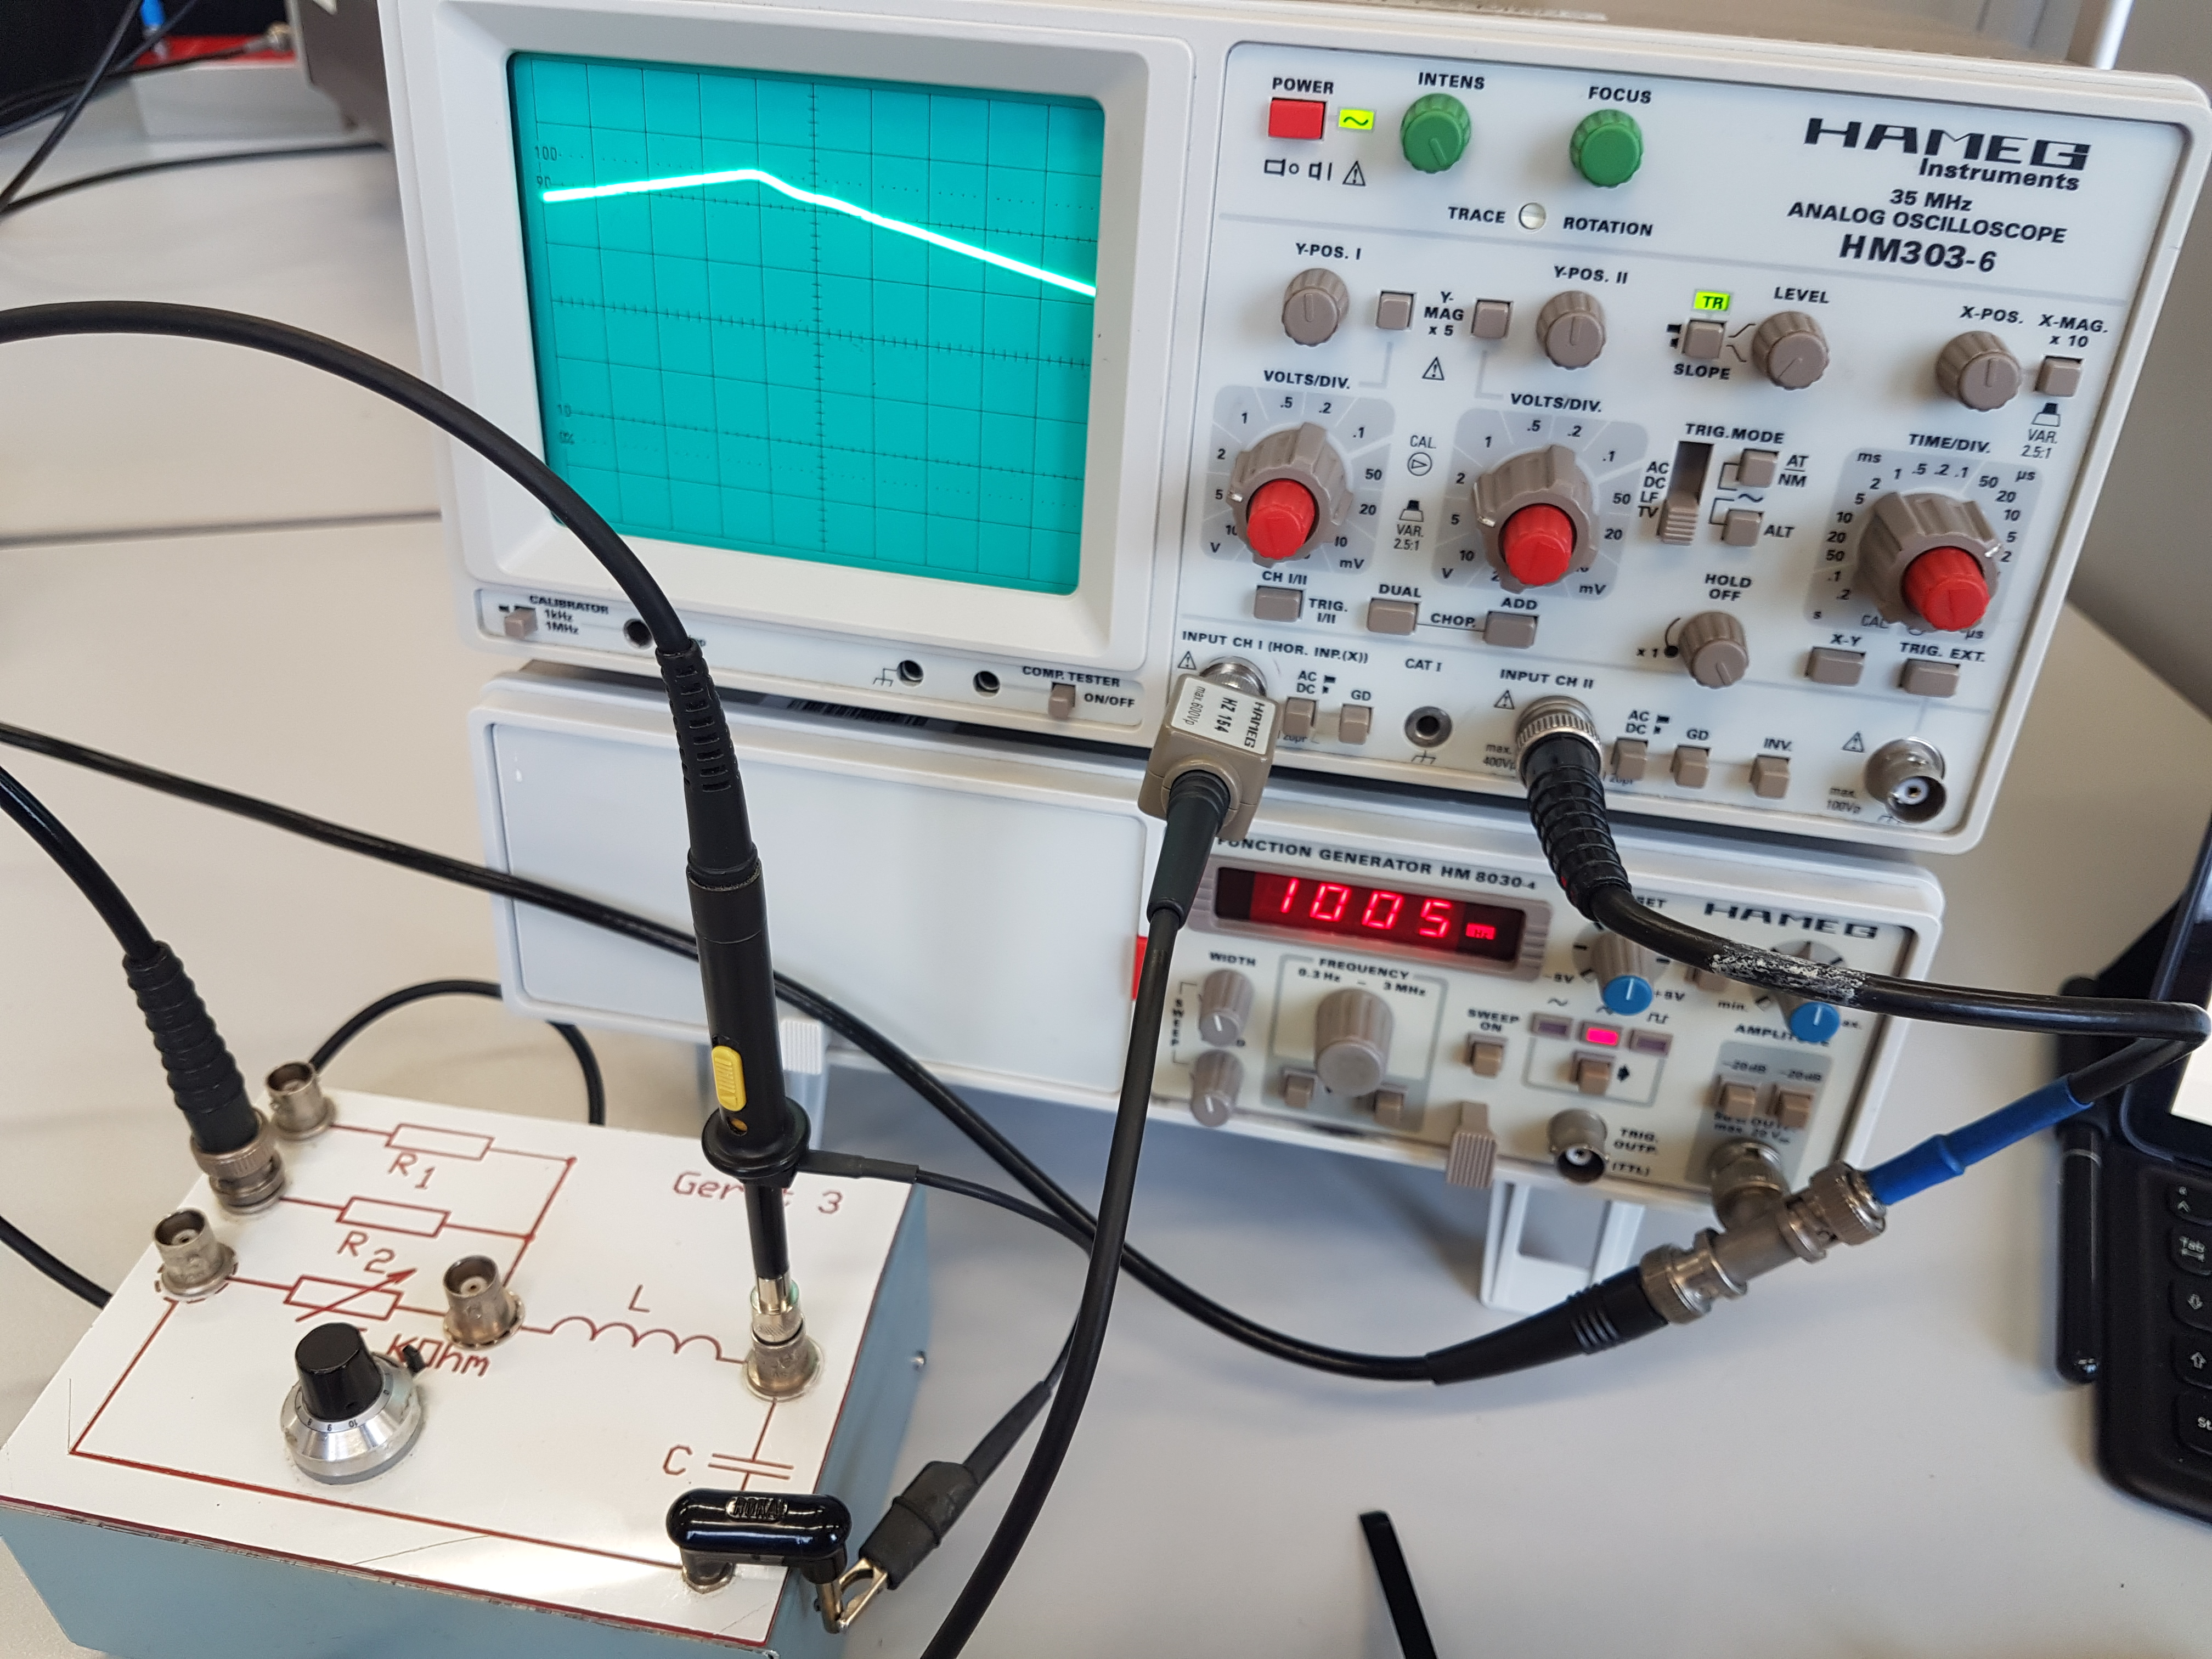
\includegraphics[width=\textwidth]{images/R2.jpg}
     \centering
     \caption{Widerstand R2}
     \label{fig:R2}
    \end{subfigure}
    \caption{Dämpfungsverhalten der Widerstände R1 und R2}
  \end{figure} 

  Die Kurven in den Bildern \ref{fig:R1} und \ref{fig:R2} spiegeln das Dämpfungsverhalten der einzelnen Widerstände wieder. 
  Es ist erkennbar, dass die Schingung in Bild \ref{fig:R2} stärker gedämpft wird, was darauf schließen lässt, dass R2 der 
  größere der beiden Widerständen ist. 

  \begin{figure}[H]
    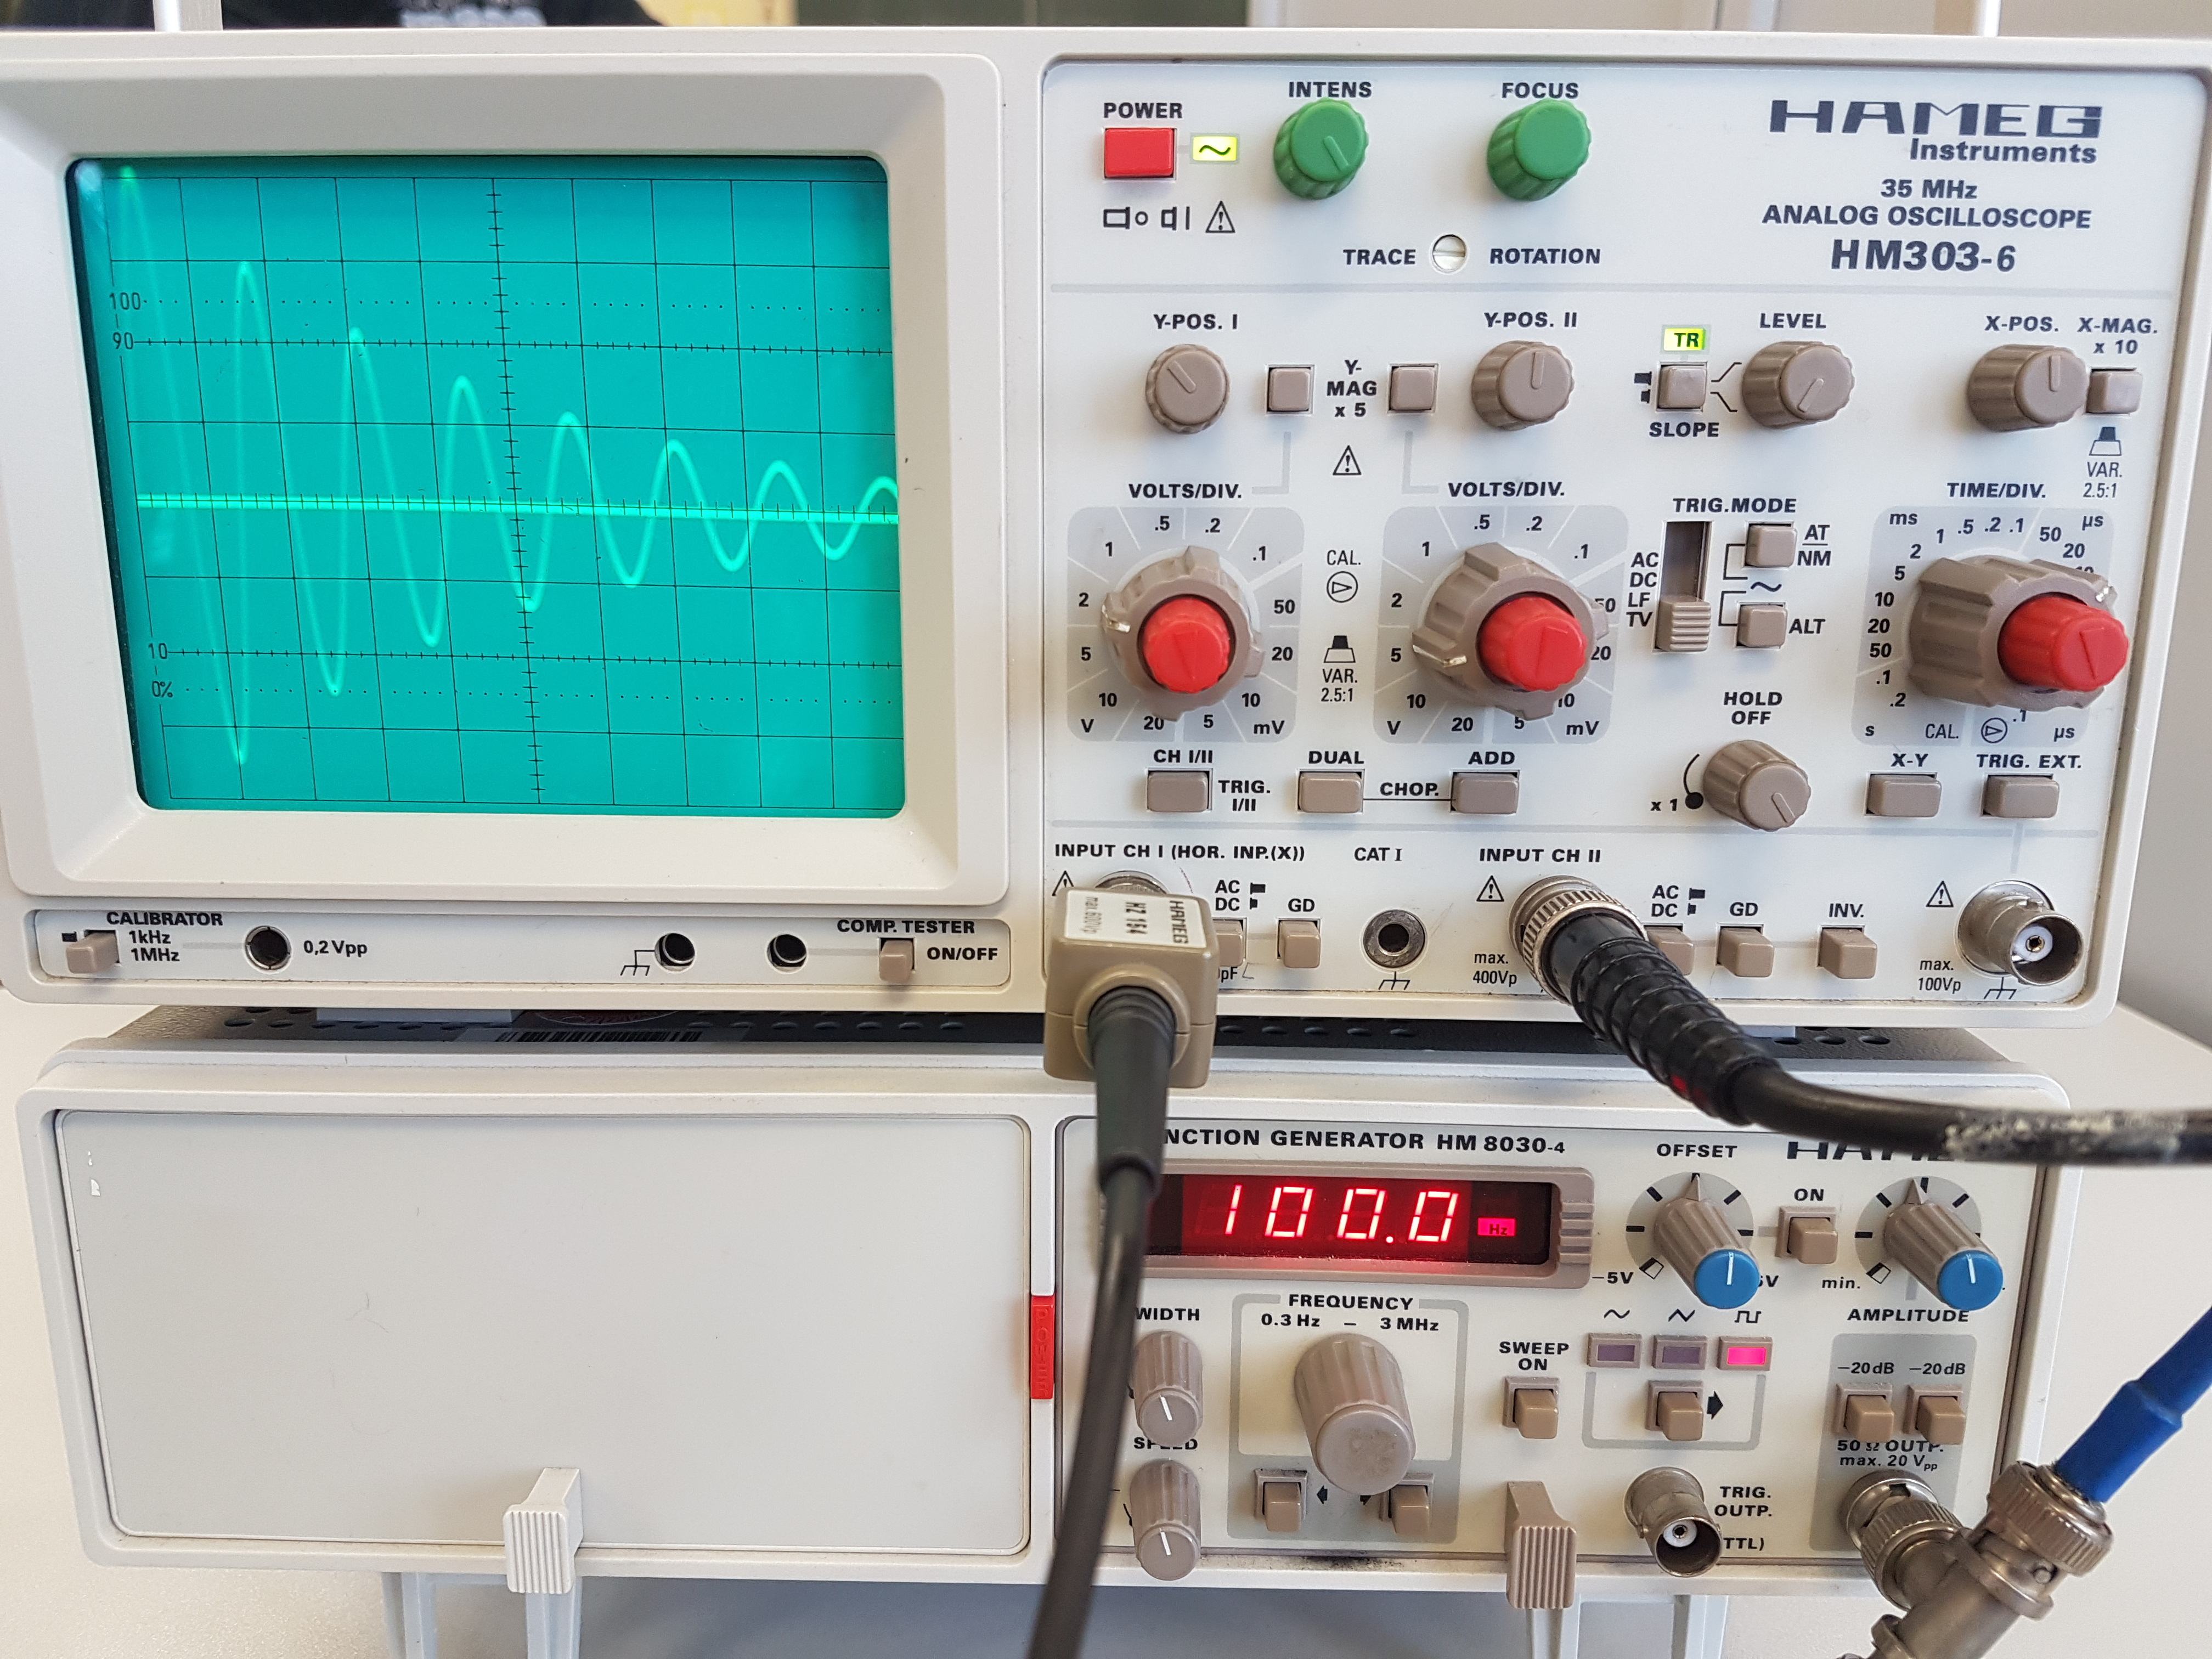
\includegraphics[width=\textwidth]{images/5a.jpg}
    \centering
    \caption{Einhüllende der Schwingungskurve}
    \label{fig:5a}
  \end{figure}

  \flushleft{Die }\justifying der Messwertpaare lässt sich der folgende Graph \ref{fig:5ajpg} beschreiben, welcher die Einhüllende 
  Die in Abbildung \ref{fig:5a} zu sehende Kurve beschreibt das Dämpfungsverhalten des LRC-Kreises bei einer angelegten Spannung von 
  10V, einem Widerstand von 271.6$\pm0.2\Omega$ und einer Frequenz von 100Hz. Aus Abbildung \ref{fig:5a} wurden die Amplituden der positiven Peaks
  abgelesen und in Tabelle \ref{tab:data_a} mit der zugehörigen Phasenverschiebung zusammengetragen.

  \begin{table}[H]
        \centering
        \caption{Messdaten von Aufg. a)}
        \input{table_a.tex} 
        \label{tab:data_a}
  \end{table}

  \flushleft{Mithilfe }\justifying der Messwertpaare lässt sich der folgende Graph \ref{fig:5ajpg} beschreiben, welcher die Einhüllende 
  Funktion $e^{+2\pi\mu t}$ des Schwingverhaltens als lineare Regression darstellt.

  \begin{figure}[H]
    \includegraphics[width=\textwidth]{build/plota.pdf}
    \centering
    \caption{Lineare Regression der Einhüllenden}
    \label{fig:5ajpg}
  \end{figure}

  $R_{eff} =$

  $T_{ex} =\text{\input{T_ex.tex}}$


%Auswertung 5b ----------------------------------------------------------------------------------------------------------------------------------------

  \flushleft{Der }\justifying aus $L$ und $C$ errechnete Widerstand beim Eintritt des aperiodischen Grenzfalls lautet:
  \begin{equation}
  R_{ap} = \text{\input{Rap.tex}} \label{Rap}
  \end{equation}
  Aus den Literaturwerten $L = \text{\input{L.tex}}$ und $C =\text{\input{C.tex}}$ ergibt sich der Widerstand 
  \begin{equation}
  R_{ap, Lit.} = \text{\input{R_ap_lit.tex}} \label{RapLit}
  \end{equation}
  Wird nun der Literaturwert mit dem errechneten Wert verglichen fällt ein relativer Fehler von
  \begin{equation}
  \frac{R_{ap} - R_{ap,Lit.}}{R_{ap,Lit.}} = \text{\input{RF_R.tex}} \label{RapAbw}
  \end{equation}
  an.

%Auswertung 5c ----------------------------------------------------------------------------------------------------------------------------------------

  
  
  \begin{table}[H]
        \centering
        \caption{Messdaten von c) und d)}
        \input{build/table_c.tex} 
        \label{tab:data_c}
  \end{table}

  \flushleft{Aus }\justifying den Messwertpaaren $(U_C, \nu)$ der Tabelle \ref{tab:data_c} werden zwei Graphen erstellt. Der erste Graph \ref{fig:4clin} 
  gibt den linearen Verlauf von Frequenz und Spannung wieder. Außerdem wurde die Breite der Resonanzkurve mit zwei vertikalen Linien eingezeichnet. 


  \begin{figure}[H]
    \begin{subfigure}{0.495\linewidth}
     \includegraphics[width=\textwidth]{build/plotclin.pdf}
     \centering
     \caption{Lineare Darstellung}
     \label{fig:4clin}
    \end{subfigure}
    \begin{subfigure}{0.495\linewidth}
     \includegraphics[width=\textwidth]{build/plotcln.pdf}
     \centering
     \caption{Logarithmische Darstellung}
     \label{fig:4cln}
    \end{subfigure}
    \caption{Resonanzkurve aus Aufg. 4c)}
  \end{figure} 

  \flushleft{Bestimmt }\justifying wurde die Breite der Resonanzkurve $\omega_+ - \omega_-$ mit $\omega = 2\cdot\pi\cdot\nu$ 
  und der Formel \eqref{eq:om+-}. Der errechneten Werte für $\omega_+ - \omega_-$ und $\omega_{+-,Lit.}$ sehen aus wie folgt:
   
  \begin{align}
  \omega_+ - \omega_- &= \text{\input{nuGraph.tex}}\\
  \omega_{+-,Lit.} &= \text{\input{nuRech.tex}}
  \end{align}
  \flushleft{Wird }\justifying $\omega_+ - \omega_-$ mit dem Literaturwert verglichen, folgt ein relativer Fehler von:
  \begin{equation}
  \frac{\omega_{+-} - \omega_{+-,Lit.}}{\omega_{+-,Lit.}} = \text{\input{RF_nu.tex}} \qquad \qquad \text{mit} \; \omega_{+-} = \omega_+ - \omega_-
  \end{equation}

  \flushleft{Aus }\justifying dem Graphen \ref{fig:4clin} und der Formel \eqref{eq:guete} ergibt sich die errechnete Resonanzüberhöhung von
  \begin{align}
  q &= \text{\input{q.tex}}
  \intertext{mit dem Literaturwert}
  q_{Lit.} &= \text{\input{q_lit.tex}}.
  \intertext{Der relative Fehler der Güte des Schwingkreises ergibt:}
  \frac{q - q_{Lit.}}{q_{Lit.}} &= \text{\input{RF_q.tex}}
  \end{align}

%Auswertung 5d ----------------------------------------------------------------------------------------------------------------------------------------

  \flushleft{Mit }\justifying den Messwertpaaren $(t, \nu)$ aus Tabelle \ref{tab:data_c} lassen sich die folgenden zwei Graphen erstellen:

  \begin{figure}[H]
    \begin{subfigure}{0.495\linewidth}
     \includegraphics[width=\textwidth]{build/plotdlin.pdf}
     \centering
     \caption{Lineare Darstellung}
     \label{fig:4dlin}
    \end{subfigure}
    \begin{subfigure}{0.495\linewidth}
     \includegraphics[width=\textwidth]{build/plotdln.pdf}
     \centering
     \caption{Logarithmische Darstellung}
     \label{fig:4dln}
    \end{subfigure}
    \caption{Resonanzkurve aus Aufg. 4d)}
  \end{figure} 

  \flushleft{Mithilfe }\justifying der Formel \eqref{eq:omegares} wird der Wert für $\nu_{res.}$ berechnet. Anhand $\nu_{res.}$
  können die Werte für $\nu_{1,2}$ bestimmt werden, indem $\nu_{res.}$ um $\sfrac{\pi}{4}$ nach oben, beziehungsweise nach unten 
  verschoben wird. Demnach folgen aus Formeln \eqref{eq:omegares} und \eqref{eq:om12} die Werte für $\nu_{1,2,res.}$ und die
  zugehörigen Literaturwerte:
  \begin{subequations}
  \begin{align}
    &\nu_1 = \text{\input{nu1.tex}} \qquad &\nu_{1,Lit.} &= \text{\input{nu1_lit.tex}}\\
    &\nu_2 = \text{\input{nu2.tex}} \qquad &\nu_{2,Lit.} &= \text{\input{nu2_lit.tex}}\\
    &\nu_{res.} = \text{\input{nu_res.tex}} &\qquad \nu_{res.,Lit.} &= \text{\input{nu_res_lit.tex}}
  \end{align}
  \end{subequations}
  \flushleft{Der }\justifying relative Fehler von $\nu_{1,2,res.}$ sieht folgendermaßen aus:
  \begin{subequations}
  \begin{align}
    \frac{\nu_1 - \nu_{1,Lit.}}{\nu_{1,Lit.}} &= \text{\input{RF_nu1.tex}}\\
    \frac{\nu_2 - \nu_{2,Lit.}}{\nu_{2,Lit.}} &= \text{\input{RF_nu2.tex}}\\
    \frac{\nu_{res.} - \nu_{res.,Lit.}}{\nu_{res.,Lit.}} &= \text{\input{RF_nu_res.tex}}
  \end{align} 
  \end{subequations}

% Diskussion %%%%%%%%%%%%%%%%%%%%%%%%%%%%%%%%%%%%%%%%%%%%%%%%%%%%%%%%%%%%%%%%%%%%%%%%%%%%%%%%%%%%%%%%%%%%%%%%%%%%%%%%%%%%%%%%%%%%%%%%%%%%%%%%%%%%%%%%%%%

\section{Diskussion}\justifying

\newpage
\nocite{V354}
\nocite{V353}
\printbibliography
\end{document}




